\documentclass{article}

\usepackage{polski}
\usepackage[utf8]{inputenc}

\usepackage{fancyhdr} % Required for custom headers
\usepackage{lastpage} % Required to determine the last page for the footer
\usepackage{extramarks} % Required for headers and footers
\usepackage[usenames,dvipsnames]{color} % Required for custom colors
\usepackage{graphicx} % Required to insert images
\usepackage{listings} % Required for insertion of code
\usepackage{courier} % Required for the courier font
\usepackage{lipsum} 
\usepackage{amsfonts}
\usepackage{amsthm}
\usepackage{hyperref}
\usepackage{tikz}
\usepackage{amsmath}
\usepackage{pdfpages}
\usepackage{hyperref}
\usepackage{mathtools}
\usepackage{enumitem}

\usepackage{amsthm}
\usepackage{epigraph}

\DeclareUnicodeCharacter{00A0}{ }

\makeatletter
\newenvironment{chapquote}[2][2em]
  {\setlength{\@tempdima}{#1}%
   \def\chapquote@author{#2}%
   \parshape 1 \@tempdima \dimexpr\textwidth-2\@tempdima\relax%
   \itshape}
  {\par\normalfont\hfill--\ \chapquote@author\hspace*{\@tempdima}\par\bigskip}
\makeatother

\newtheorem{thm}{Twierdzenie}
\newtheorem{remark}{Uwaga}
\newtheorem{lemat}{Lemat}
\newtheorem{wniosek}{Wniosek}
\newtheorem{definicja}{Definicja}
\newtheorem{ciekawostka}{Ciekawostka}
\newtheorem{przyklad}{Przykład}
\newtheorem{fakt}{Fakt}



\newenvironment{prooff}{\paragraph{Dowód:}}{\hfill$\square$}
\newenvironment{rozw}{\paragraph{Rozwiązanie:}}{\hfill}


\usepackage{inconsolata} % very nice fixed-width font included with texlive-full
\usepackage[usenames,dvipsnames]{color} % more flexible names for syntax highlighting colors
\usepackage{listings}

\usepackage[T1]{fontenc}
\usepackage[scaled=0.84]{beramono}
\usepackage[utf8]{inputenc}
\usepackage[x11names]{xcolor}
\usepackage{listings}
\lstnewenvironment{CPP}
 {\lstset{language=C++,
    basicstyle=\small\ttfamily,
    keywordstyle=\bfseries,
    identifierstyle=\color{red},
    commentstyle=\color{brown},
    stringstyle=\color{blue},
    tabsize=2,
}}{}

% Margins
\topmargin=-0.45in
\evensidemargin=0in
\oddsidemargin=0in
\textwidth=6.0in
\textheight=9.0in
\headsep=0.25in

\linespread{1.1} % Line spacing

% Set up the header and footer
\pagestyle{fancy}
\lhead{\hmwkAuthorName} % Top left header
\rhead{\firstxmark} % Top right header
\lfoot{\lastxmark} % Bottom left footer
\cfoot{} % Bottom center footer
\renewcommand\headrulewidth{0.4pt} % Size of the header rule
\renewcommand\footrulewidth{0.4pt} % Size of the footer rule

\setlength\parindent{0pt} % Removes all indentation from paragraphs
%----------------------------------------------------------------------------------------
%	DOCUMENT STRUCTURE COMMANDS
%	Skip this unless you know what you're doing
%----------------------------------------------------------------------------------------

% Header and footer for when a page split occurs within a problem environment
\newcommand{\enterProblemHeader}[1]{
\nobreak\extramarks{#1}{#1 continued on next page\ldots}\nobreak
\nobreak\extramarks{#1 (continued)}{#1 continued on next page\ldots}\nobreak
}

% Header and footer for when a page split occurs between problem environments
\newcommand{\exitProblemHeader}[1]{
\nobreak\extramarks{#1 (continued)}{#1 continued on next page\ldots}\nobreak
\nobreak\extramarks{#1}{}\nobreak
}

\setcounter{secnumdepth}{0} % Removes default section numbers
\newcounter{homeworkProblemCounter} % Creates a counter to keep track of the number of problems

\newcommand{\homeworkProblemName}{}
\newenvironment{homeworkProblem}[1][Zadanie \arabic{homeworkProblemCounter}]{ % Makes a new environment called homeworkProblem which takes 1 argument (custom name) but the default is "Problem #"
\stepcounter{homeworkProblemCounter} % Increase counter for number of problems
\renewcommand{\homeworkProblemName}{#1} % Assign \homeworkProblemName the name of the problem
\section{\homeworkProblemName} % Make a section in the document with the custom problem count
\enterProblemHeader{\homeworkProblemName} % Header and footer within the environment
}{
\exitProblemHeader{\homeworkProblemName} % Header and footer after the environment
}

\newcommand{\problemAnswer}[1]{ % Defines the problem answer command with the content as the only argument
\noindent\framebox[\columnwidth][c]{\begin{minipage}{0.98\columnwidth}#1\end{minipage}} % Makes the box around the problem answer and puts the content inside
}

\newcommand{\homeworkSectionName}{}
\newenvironment{homeworkSection}[1]{ % New environment for sections within homework problems, takes 1 argument - the name of the section
\renewcommand{\homeworkSectionName}{#1} % Assign \homeworkSectionName to the name of the section from the environment argument
\subsection{\homeworkSectionName} % Make a subsection with the custom name of the subsection
\enterProblemHeader{\homeworkProblemName\ [\homeworkSectionName]} % Header and footer within the environment
}{
\enterProblemHeader{\homeworkProblemName} % Header and footer after the environment
}

\usepackage{listings} % Required for inserting code snippets
\usepackage[usenames,dvipsnames]{color} % Required for specifying custom colors and referring to colors by name

\definecolor{DarkGreen}{rgb}{0.0,0.4,0.0} % Comment color
\definecolor{highlight}{RGB}{255,251,204} % Code highlight color

% Create a command to cleanly insert a snippet with the style above anywhere in the document
\newcommand{\insertcode}[2]{\begin{itemize}\item[]\lstinputlisting[caption=#2,label=#1,style=Style1]{#1}\end{itemize}} % The first argument is the script location/filename and the second is a caption for the listing

%----------------------------------------------------------------------------------------
%	NAME AND CLASS SECTION
%----------------------------------------------------------------------------------------

\newcommand{\hmwkTitle}{Problem palaczy tytoniu} % Assignment title
\newcommand{\hmwkDueDate}{} % Due date
\newcommand{\hmwkClass}{Systemy operacyjne} % Course/class
\newcommand{\hmwkClassTime}{} % Class/lecture time
\newcommand{\hmwkClassInstructor}{} % Teacher/lecturer
\newcommand{\hmwkAuthorName}{Bartosz Bednarczyk - obowiązkowe zadanie z systemów operacyjnych} % Your name

%----------------------------------------------------------------------------------------

\begin{document}
 
\title{Doświadczalne określenie długości bloku pamięci podręcznej}
\date{\today}
\author{Bartosz Bednarczyk}
 
\maketitle
 
\subsection*{Krótki wstęp teoretyczny}
 
Pamięć podręczna procesora to pamięć statyczna o krótkim czasie dostępu. Zlokalizowana jest często bezpośrednio w jądrze procesora. Ma ona wielopoziomową budowę, dzięki czemu zapewnia złudzenie posiadania szybciej i pojemnej pamięci głównej. Zmniejsza również średni czas dostępu do pamięci głównej. Nas interesować będzie pamięć tzw. pierwszego poziomu, którą dalej będę nazywał w skrócie pamięcią $L1$. Charakteryzuje się ona najszybszym dostępem wśród innych poziomów kaszu.
 
\subsection*{Ciekawe fakty o pamięci $L1$}
 
Spośród wielu informacji o kaszu uznałem, że interesujące są następujące fakty:
 
\begin{itemize}
\item L1 jest zawsze zintegrowana z rdzeniem procesora, a więc taktowana tą samą częstotliwością, działająca z tą samą szybkością; 
\item  L1 ma decydujący wpływ na wydajność systemu;
\item Dzięki pamięci $L1$ znacznie rzadziej musi się odwoływać do wolnej pamięci RAM.
\end{itemize}
 
\subsection{Jak sprawdzić informacje na temat pamięci na swoim komputerze?}
 
Nic prostszego. Wystarczy wpisać polecenie \textbf{sysctl hw}. Część wydruku z mojego komputera można zaobserwować poniżej. Szczególną uwagę należy zwrócić na fragment zaznaczony niebieskim kolorem.
 
\begin{figure}[h!]
\centering
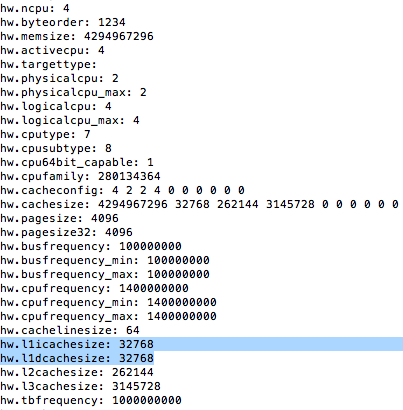
\includegraphics[scale=0.5]{kaszinfo}  
\end{figure}
 
\subsection{Zrób to sam!}
 
Ciekawym pomysłem jest to, by samemu pobawić się w mierzenie długości bloku kaszu. Napisałem w tym celu program komputerowy (w języku C), który przez wielokrotne testy oraz ich uśrednianie,   sugerował nam żądany rozmiar.
Przedstawię najpierw z jakich narzędzi będę korzystał w kodzie.
 
\begin{itemize}
\item \textbf{Wędrowanie po tablicy (array walker)}. Tworzymy jednowymiarową tablicę 32-bitowych słów o $N$ elementach, nazywamy ją ,,array'' . Tablica zaczyna się pod adresami podzielnymi przez rozmiar strony i ma rozmiar wielokrotności rozmiaru strony. Mamy zbiór $S$ wszystkich indeksów tej tablicy. Chcemy wygenerować pewne szczególne permutacje zbioru $S$. Po zakodowaniu permutacji, uruchamiamy procedurę array\_walker. Przechodzi ona po kolejnych elementach tablicy i generuje odczyty pamięci (i potencjalne chybienia). Procedura kończy się po osiągnięciu    ostatniego elementu ciągu lub po przejrzeniu $N$ elementów, gdy permutacja była cyklem.
 
\item \textbf{Zatruwanie pamięci podręcznej}. W niektórych przypadkach należy zapełnić pamięć podręczną pewnymi danymi w taki sposób, aby każdy kolejny odczyt innych danych generował chybienie. Dzięki temu, w pewnym sensie ,,opróżniamy'' pamięć podręczną. Określa się to mianem ,,zatruwania pamięci podręcznej''. Zadanie to realizuje procedura ,,poison\_cache''.
 
\item \textbf{ Pobieranie czasu (timer\_*)}. Chcemy mierzyć czas z dokładnością do milisekund. Służy do tego zestaw procedur timer\_init, timer\_start, timer\_stop, timer\_print.
 
\end{itemize}
 
Algorytm programu wygląda następująco:
 
\begin{enumerate}
    \item Utwórz dostatecznie dużą tablicę (rozmiar musi być potęgą dwójki).
    \item Zatruj kasz.
    \item Następnie dla $n \in \lbrace 1,2,3, \ldots, N\footnote{Liczba testów kontrolnych - u mnie jest to 37.} \rbrace$ powtarzaj:
    \begin{enumerate}
        \item Zatruj kasz.
        \item Zacznij odmierzać czas.
        \item Wielokrotnie wędruj po elementach tablicy, zapełniając je przykładowymi wartościami (np. jedynką), ,,skacząc'' co $n$ elementów.
        \item Zatrzymaj czas i podaj ile czasu upłynęło.
    \end{enumerate}
    \item Zakończ program.
   
\end{enumerate}
 
Kiedy wykonamy program wielokrotnie i uśrednimy otrzymane wyniki, to możemy spróbować wywnioskować z nich rozmiar bloku pamięci podręcznej. Wynik moich eksperymentów poniżej.
 
\begin{table}[h!]
\centering
\label{my-label}
\begin{tabular}{|c|c|c|c|c|c|c|c|c|c|c|c|c|c|c|c|c|}
\hline
1    & 2     & 3     & 4    & 5    & 6    & 7    & 8    & 9    & 10   & 11   & 12   & 13   & 14   & 15   & 16            & 17   \\ \hline
0.90 & 0.884 & 0.882 & 0.87 & 0.93 & 1.55 & 1.81 & 2.03 & 2.31 & 2.56 & 2,79 & 3.01 & 3.24 & 3.53 & 3.79 & \textbf{4,16} & 4,17 \\ \hline
18   & 19    & 20    & 21   & 22   & 23   & 24   & 25   & 26   & 27   & 28   & 29   & 30   & 31   & 32   & 33            & 34   \\ \hline
4,10 & 4,14  & 4,21  & 4,17 & 4,14 & 4,18 & 4,16 & 4,13 & 4,19 & 4,14 & 4,15 & 4,23 & 4,14 & 4,19 & 4,30 & 4,21          & 4,20 \\ \hline
\end{tabular}
\end{table}
 
Z przedstawionej tabeli można wyczytać, że początkowo czas przechodzenia po tablicy był stosunkowo niewielki. Rośnie on wraz ze wzrostem $N$. W pewnym momencie czas się stabilizuje i wyniki obliczeń są w miarę podobne. Od czego to zależy? \pagebreak
 
Okazuje się, że czas przechodzenia po tablicy ma ścisły związek z rozmiarem kaszu. Od podanego $N$ zależy, czy wszystkie elementy, po których przechodzimy, mieszczą się w pamięci podręcznej czy nie. Jeżeli nie, to program musi doczytywać elementy na bieżąco i wyrzucać stare dane z pamięci, które za chwilę znowu będą zmieniane. Przy $N$ mniejszych od rozmiaru długości bloku kaszu, taka sytuacja nie występuje. \\
 
Możemy więc wywnioskować, że idealnym kandydatem na ,,zbilansowanie'' wyników byłoby $N = 16$, gdyż dla $N > 16$ wyniki były w miarę podobnie, a w poprzednich iteracjach czasy gwałtownie rosły. Obliczając formułę, $16 * sizeof(int) * sizeof(int)$ dostajemy liczbę $64$, co zgadza się z wyświetlonym komunikatem systemowym z pierwszej strony sprawozdania (patrz: hw.cachelinesize). \\
 
Udało nam się zatem policzyć długość bloku kaszu bez używania specjalistycznych narzędzi.
 
\subsection*{Dodatek. Kod źródłowy funkcji ,,measure''}
 
Do sprawozdania załączam również kod źródłowy funkcji ,,measure'' napisany w języku C, który realizuje algorytm opisany na poprzedniej stronie.\\
 
\lstset{inputencoding=utf8}
\lstinputlisting[language=C++]{measure.c}
 
 
 
\end{document}